\documentclass{beamer}
\usefonttheme{serif} % default family is serif
\usepackage{graphicx}
\usepackage{xcolor}
\usepackage{colortbl}
\usepackage{multirow,tabularx}
\usepackage{tikz}
\usepackage{hyperref}
\usepackage{physics}
\usepackage{siunitx}

% Code listing
\usepackage{listings}
\usepackage{xcolor}

% Define Python syntax highlighting
\lstdefinelanguage{python}{
	morekeywords={if, else, for, while, def, return, import, print, lambda, in, True, False, and, or, not, try, except, class},
	morecomment=[l]{\#},
	morestring=[b]",
	morestring=[b]',
	sensitive=true
}

% Define listing style
\lstset{
	language=python,
	basicstyle=\ttfamily\small,
	keywordstyle=\color{blue}\bfseries,
	commentstyle=\color{gray},
	stringstyle=\color{red},
	numbers=left,
	numberstyle=\tiny\color{gray},
	stepnumber=1,
	numbersep=5pt,
	breaklines=true,
	breakatwhitespace=true,
	frame=single,
	backgroundcolor=\color{lightgray!20},
	tabsize=2
}

\usepackage{amsthm}
\usepackage{amsmath}

% Blue theme for the presentation
\definecolor{purple}{rgb}{0.3, 0.0, 0.557}
\definecolor{blue}{rgb}{0.0234375, 0.11328125, 0.609375}

\setbeamercolor{frametitle}{fg=blue}
\setbeamercolor{title}{fg=blue}
\setbeamercolor{structure}{fg=blue}

\title{\textcolor{blue}{Introduction to Programming for AI}}
\subtitle{\textcolor{blue}{Wigner Summer Camp \\ Data and Compute Intensive Sciences Research Group}}
\author{\textcolor{blue}{Balázs, Paszkál, Vince, Levente, Antal \\ Éva, Hajni}}

\date{\textcolor{blue}{7-11 July 2025}}

% Footline with slide number
\setbeamertemplate{footline}
{
	\leavevmode%
	\hbox{%
		\begin{beamercolorbox}[wd=.1\paperwidth,ht=2.25ex,dp=1ex,left]{page number in head/foot}%
			\hspace{1em} \textcolor{blue}{\insertframenumber}%
	\end{beamercolorbox}}%
	\vskip0pt%
}

\begin{document}
	
	\begin{frame}
		\titlepage
		\begin{columns}
			\centering
			\column{0.3\textwidth}
			\column{0.3\textwidth}
			\centering
			
\includegraphics[width=0.8\textwidth]{img/logo.png}
			\column{0.3\textwidth}
		\end{columns}
	\end{frame}
	
	\begin{frame}{Course Overview}
		This course will cover essential programming tools for AI:
		\begin{itemize}
			\item Core Python programming
			\item Numerical computing with NumPy
			\item Data manipulation with pandas
			\item Data visualization with matplotlib
			\item Deep learning basics with PyTorch
		\end{itemize}
		
		Each topic has:
		\begin{itemize}
			\item Lecture notebook (e.g., python\_basics.ipynb)
			\item Solution notebook (e.g., python\_basics\_solutions.ipynb)
		\end{itemize}
	\end{frame}
	
	\begin{frame}{Why Python for AI?}
	    \begin{itemize}
			\item \textbf{Readability:} Simple syntax similar to pseudocode
			\item \textbf{Ecosystem:} Rich collection of libraries for scientific computing
			\item \textbf{Community:} Large user base and extensive documentation
			\item \textbf{Flexibility:} Supports both prototyping and production
		\end{itemize}
	
		\begin{example}[Simple Python Example]
			\begin{lstlisting}
				# Calculate factorial
				def factorial(n):
				return 1 if n == 0 else n * factorial(n-1)
			\end{lstlisting}
		\end{example}
	\end{frame}
	
	\begin{frame}{Python Basics}
		Core concepts you'll learn:
		\begin{itemize}
			\item Variables and data types (int, float, str, bool)
			\item Control flow (if-else, for/while loops)
			\item Functions and lambda expressions
			\item Lists, tuples, dictionaries, sets
			\item Object-oriented programming basics
		\end{itemize}
		
		\begin{example}[List Comprehension Example]
			\begin{lstlisting}
				squares = [x**2 for x in range(10)]
			\end{lstlisting}
		\end{example}
	\end{frame}
	
	\begin{frame}{NumPy: Numerical Computing}
		\begin{itemize}
			\item \textbf{What:} Fundamental package for scientific computing
			\item \textbf{Why:} Efficient array operations and linear algebra
			\item \textbf{Key features:}
			\begin{itemize}
				\item N-dimensional array object
				\item Broadcasting functions
				\item Linear algebra, Fourier transform, random number capabilities
			\end{itemize}
		\end{itemize}
		
		\begin{example}[NumPy array]
			\begin{lstlisting}
				import numpy as np
				a = np.array([[1, 2], [3, 4]])
				b = np.ones((2,2))
				c = a + b  # Element-wise addition
			\end{lstlisting}
		\end{example}
	\end{frame}
	
	\begin{frame}{pandas: Data Analysis}
		\begin{itemize}
			\item \textbf{What:} Powerful data manipulation library
			\item \textbf{Why:} Essential for data cleaning and preprocessing
			\item \textbf{Key features:}
			\begin{itemize}
				\item DataFrame object (like Excel tables)
				\item Handling missing data
				\item Merging and joining datasets
				\item Time series functionality
			\end{itemize}
		\end{itemize}
		
		\begin{example}[pandas DataFrame]
			\begin{lstlisting}
				import pandas as pd
				data = {'Name': ['Alice', 'Bob'], 'Age': [25, 30]}
				df = pd.DataFrame(data)
			\end{lstlisting}
		\end{example}
	\end{frame}
	
	\begin{frame}{matplotlib: Data Visualization}
		\begin{itemize}
			\item \textbf{What:} Comprehensive 2D plotting library
			\item \textbf{Why:} Visualize data and model results
			\item \textbf{Key features:}
			\begin{itemize}
				\item Publication-quality figures
				\item Various plot types (line, bar, scatter, histogram)
				\item Customizable styling
			\end{itemize}
		\end{itemize}
		
		\begin{example}[Simple plot]
			\begin{lstlisting}
				import matplotlib.pyplot as plt
				plt.plot([1, 2, 3], [1, 4, 9])
				plt.xlabel('X axis')
				plt.ylabel('Y axis')
			\end{lstlisting}
		\end{example}
	\end{frame}
	
	\begin{frame}{PyTorch: Deep Learning}
		\begin{itemize}
			\item \textbf{What:} Open-source machine learning library
			\item \textbf{Why:} Flexible architecture for research and production
			\item \textbf{Key features:}
			\begin{itemize}
				\item Tensor computation with GPU acceleration
				\item Automatic differentiation
				\item Neural network building blocks
			\end{itemize}
		\end{itemize}
		
		\begin{example}[Simple tensor operation]
			\begin{lstlisting}
				import torch
				x = torch.tensor([[1, 2], [3, 4.]])
				y = torch.matmul(x, x)  # Matrix multiplication
			\end{lstlisting}
		\end{example}
	\end{frame}
	
	\begin{frame}{How These Tools Work Together}
		\begin{center}
			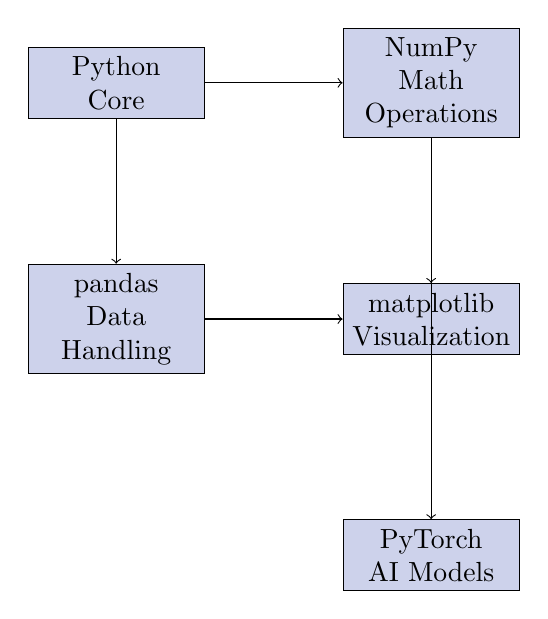
\begin{tikzpicture}[node distance=2cm]
				\node (python) [draw, fill=blue!20, text width=2cm, align=center] {Python\\Core};
				\node (numpy) [draw, fill=blue!20, text width=2cm, align=center, right of=python, xshift=2cm] {NumPy\\Math Operations};
				\node (pandas) [draw, fill=blue!20, text width=2cm, align=center, below of=python, yshift=-1cm] {pandas\\Data Handling};
				\node (matplotlib) [draw, fill=blue!20, text width=2cm, align=center, below of=numpy, yshift=-1cm] {matplotlib\\Visualization};
				\node (pytorch) [draw, fill=blue!20, text width=2cm, align=center, below of=matplotlib, yshift=-1cm] {PyTorch\\AI Models};
				
				\draw [->] (python) -- (numpy);
				\draw [->] (python) -- (pandas);
				\draw [->] (numpy) -- (matplotlib);
				\draw [->] (pandas) -- (matplotlib);
				\draw [->] (numpy) -- (pytorch);
			\end{tikzpicture}
		\end{center}
	\end{frame}
	
	\begin{frame}{Practical Workflow Example}
		\begin{enumerate}
			\item Load and clean data with pandas
			\item Perform numerical operations with NumPy
			\item Visualize results with matplotlib
			\item Build and train models with PyTorch
			\item Analyze results and iterate
		\end{enumerate}
		
		\begin{example}[AI workflow]
			\begin{lstlisting}
				# 1. Load data
				data = pd.read_csv('dataset.csv')
				
				# 2. Preprocess
				X = data[['feature1', 'feature2']].values
				y = data['target'].values
				
				# 3. Build model
				model = torch.nn.Linear(2, 1)
			\end{lstlisting}
		\end{example}
	\end{frame}
	
	\begin{frame}{Getting Started}
		\begin{itemize}
			\item Install Python (recommend Anaconda distribution)
			\item Jupyter Notebook for interactive coding
			\item Course materials available on GitHub
			\item Exercises with solutions for practice
		\end{itemize}
		
		\begin{block}{Next Steps}
			\begin{itemize}
				\item Start with python\_basics.ipynb
				\item Progress through each module
				\item Ask questions and experiment!
			\end{itemize}
		\end{block}
	\end{frame}
	
\end{document}